\documentclass[10pt, a4paper]{article}
\usepackage{amsmath}
\usepackage{amsfonts}
\usepackage[english]{babel}
\usepackage[utf8]{inputenc}
\usepackage{color}
\usepackage{graphicx}
\usepackage[version=4]{mhchem}
\usepackage{rotating}
\renewcommand{\baselinestretch}{1}
\usepackage{fullpage}
\usepackage{mathtools}
\usepackage{caption}
\usepackage{tikz}
\usepackage{standalone}
\usepackage{subfigure}
\usetikzlibrary{decorations.pathreplacing}
\usetikzlibrary{arrows}
\usetikzlibrary{fadings}
%\usepackage{parskip}
\usepackage{import}
\usepackage{authblk}
%\setlength{\parindent}{0pt}


\begin{document}

\title{IPSW - Modelling Change of Website Archives}
% \author{Caoimhe Rooney, Ian Roper, Jessica Williams, Ian Milligan, Nathan Taback}
\author[1]{Caoimhe Rooney}
\author[1]{Ian Roper}
\author[1]{Jessica Williams}
\author[2]{Ian Milligan}
\author[3]{Nathan Taback}
\affil[1]{Mathematical Institute, University of Oxford}
\affil[2]{Department of History, University of Waterloo}
\affil[3]{Department of Statistical Sciences and Computer Science, University of Toronto}
\date{}
\maketitle

\vspace{-12mm}

\section{Problem and Aims}

\vspace{-2mm}

 Web archives, collections of old websites dating back to the mid-1990s that have been collected by institutions like the Internet Archive and libraries around the world, are invaluable research objects.
 They often consist of website domains (i.e. \texttt{www.domain.com} or \texttt{www.cnn.com}) which have been ``crawled'' by a web archival institution, which obtains all of the information on a given domain on a particular date.
 The scale of all this data is overwhelming for researchers to be able to extract the relevant data from the large number of crawls.
 Being able to find where large changes to the domain occurred in time so that the crawls performed on these dates can be investigated further would be of significant use for historians, as for example they could find particular websites amongst hundreds of domain snapshots to examine.
 Furthermore, the libraries which crawl the websites and store the archives have a data `allowance' which the cost of each crawl is taken out of.
 Therefore, for example, a librarian might be interested in crawling a website that is updated more frequently more often; conversely, a website that is rarely updated might be crawled less.
 In other words, more information would help guide crawling decisions. 
 
 In our project, we find (from existing literature, for example \cite{dhyani2002survey}) or create different metrics for quantifying change between websites.
 We then apply these metrics to a web domain crawled from several different dates, comparing two consecutive crawls.
 This allows us to produce a time series of how much the website has changed from the previous crawl.
 We then compare the different metrics against each other, and attempt to identify large changes of the organisation behind the website which we know occurred in the past.
\vspace{-3mm}

\section{Text}
\label{sec:text}
\vspace{-2mm}
 We obtain the plain text (i.e. what appeared on all of the HTML pages) from the domain homepage for every crawl.
 Our goal is to compare the text from one crawl to the next and quantify how much the text has changed between them.
 There are a variety of metrics within the literature, in particular we explore the metrics described by Kwon \textit{et~al.}
 \cite{kwon2006precise}.
 All the metrics are normalised to have a quantity between zero and one such that a crawl of a page that was identical to the last crawl should return a score of zero, and a crawl of a page that has absolutely nothing in common with the previous crawl should return one.
\vspace{-2mm}
\subsection{Metrics}
\vspace{-2mm}
\textit{\textbf{Byte-wise comparison metric}}:
 This technique compares two webpages sequentially character by character.
 The metric then returns one if any change has occurred and zero otherwise \cite{brewington2000dynamic, cho1999evolution,kim2005empirical}.
 A one is returned for even very trivial changes, for example, adding a blank space.
 Therefore, this metric is over-sensitive and does not provide particularly meaningful insight into the change between two strings of text.
 However, the byte-wise metric is useful in limiting the pages of interest, namely, if the metric is zero for any crawl, we know that there have been absolutely no changes at all and hence we need not explore this crawl further.
\vspace{1.5mm}

\noindent \textit{\textbf{TF.IDF cosine distance}}:
 TF.IDF is shorthand for ``term frequency-inverse document frequency'' and is used to quantify how important a word is to a document of text.
 The underlying concept is that relevant words are not necessarily the most frequent words.
 For example, if considering book reviews, the words ``character'' or ``plot'' might appear very frequently, but do not give valuable insight to summarise the review.
 This metric is calculated by finding the term frequency (TF) of a word, namely the frequency of a word in a document.
 We also find the inverse document frequency (IDF) of a word, which is the measure of how significant that term is in the collection of documents.
 By combining these concepts, we obtain TF.IDF weighted vectors to represent the content of each document and the metric value is calculated as the cosine distance between them \cite{salton1986introduction}.
 TF.IDF has evident success in search engine algorithms to shift the definition of word-value from frequency to relevance \cite{beel2016paper}.

%\begin{equation}
%D_{\cos} = 1-\frac{\boldsymbol{p}\cdot \boldsymbol{p}'}{||\boldsymbol{p}||_2||\boldsymbol{p}'||_2}.
%\end{equation}
\vspace{1.5mm}
\noindent \textit{\textbf{Word distance}}:
 The word distance metric calculates the number of words in a document that have changed \cite{ntoulas2004s}.
 This is done by counting the number of common words in each document and normalising with respect to the total number of words in the two documents.
 Although less sensitive than byte-wise, both TF.IDF and the word distance metric are unable to account for change in word order. 
%	D_{WD} = 1- \frac{2\cdot\vert\text{common words}\vert}{m+n},
%\end{equation}

\vspace{1.5mm}
\noindent \textit{\textbf{Levenshtein distance}}:\\
 The Levenshtein distance between two strings is the minimum number of single character edits, (substitutions, insertions or deletions) required to transform one string into the other \cite{levenshtein1996}.
 For example, the Levenshtein distance between ``test'' and ``tent'' is 1, due to the single substitution of ``s'' to ``n''.
 We calculated the Levenshtein distance between the text of two webpages and normalised this value according to the maximum Levenshtein distance: the length of the longer string. 
\vspace{-3mm}

\section{Hyperlinks}
\label{sec:links}
\vspace{-2mm}
 There are two ways in which we use the hyperlinks of a web domain to quantify the change between the domain from different crawls.
 The first of which is to compare the hyperlinks from the domain to pages of external domains.
 For simplicity, we only consider hyperlinks on the homepage of the domain pointing to webpages of external domains and we do not consider the frequency of each hyperlink, only whether the hyperlink exists or not.
 Our method for quantifying the change in external hyperlinks is similar to that of the word distance method.
 We divide the total number of links that are present in the two different crawls of the domain and normalise this by the average number of hyperlinks on the homepage of the domain from both crawls.
 We believe that links to external websites would be of particular interest to the creators of a domain as they are linking to other organisations which they are passionate about.
 Therefore, if these links change, it would suggest a large change in the focus of the domain.
 
 The second method we use is to represent all of the webpages in a domain as nodes in a network which are connected by directed edges representing hyperlinks from one webpage to another.
 This network representing the structure of a domain may change from one crawl to the next, when webpages are added and removed from a domain between two crawls or when hyperlinks within a domain change.
 Several global metrics to quantify the change between these networks have been proposed, including compactness and stratum, which are explained in detail by Botafogo \textit{et al.} in \cite{botafogo1992structural}.
 Depending on the structural changes that are to be detected or expected from the domain, these different metrics can be more or less useful.
 Unfortunately, at the time of writing, we do not have sufficient webpage data to perform this analysis on the data from the NDP domain data, however, we hope to be able to continue this work once the data is able to be obtained.
\vspace{-3mm}

\section{Thumbnails}
\label{sec:images}
\vspace{-2mm}
 In addition to changes in website text and structure, meaningful change in domain is often reflected by a change in the visual structure of the page.
 We can generate a website snapshot of one of the webpage crawls using the Wayback Machine (\texttt{www.archive.org/web}) which holds one of the web archives.
 Hence, a promising approach to quantify the change in a web domain, is by applying image analysis techniques to detect the similarity between webpage thumbnails \cite{alsum2014thumbnail}.
 This has previously been considered for pairs of images, although plotting similarity over time has yet to be considered.
 Several methods for comparing thumbnails have been proposed and implemented previously \cite{henzinger,broder,manku}, and an accessible summary is provided in \cite{alsum2014thumbnail}.
 
 Some image comparison techniques may not always produce meaningful results -- e.g., images on a homepage may change frequently, with no change in website content.
 Therefore, we propose the use of the structural similarity index (SSIM) \cite{ssim}, which measures the similarity between two images by comparing average pixel intensity in various sub-windows of the page.
 The SSIM value is between $-1$ and $1$ so in order to compare this metric with the text and hyperlink metrics, we scale the SSIM value to lie between zero and one, and call this metric, $d$.

\begin{figure}[h!]
\centering
\def\svgwidth{
0.7\columnwidth}
\import{report-images/}{all-waybacks.pdf_tex}
  \caption{Three image comparisons from \texttt{www.ndp.ca}.}
\label{fig::wayback_images}
\end{figure}

 Our \texttt{python} code automatically generates thumbnails of the homepage of all crawls of a chosen domain recorded in the Wayback Machine, and uses this to obtain a library of 108 thumbnails from \texttt{www.ndp.ca} from 2005-2019.
 There were times when the Wayback Archive had only saved a page that had failed to render, which presented itself as a primarily white webpage.
 We detected these `fails' and removed them from the data set by imposing a maximum percentage of white pixels (80\%).
 In Figure \ref{fig::wayback_images}, we display an example of a failed render, as well as two different timesteps which demonstrate visually the value of the SSIM metric.
\vspace{-3mm}

\section{Results}

 Results for all metrics considered in this report are plotted in Figure \ref{fig:results} for data obtained from \texttt{www.ndp.ca}.
 Figure \ref{fig:text} displays the four text metrics described in Section \ref{sec:text}, and we see that all metrics follow a similar pattern of peaks and troughs with the exception of the Byte-wise metric.
 This is due to it only taking values of zero or one as explained in Section \ref{sec:text}.
 The image comparison, using the SSIM metric described in Section \ref{sec:images} and scaled appropriately is plotted in Figure \ref{fig:image}.
 The section of missing data corresponds to a time interval when the wayback archive failed to generate a representative thumbnail (see Section Figure \ref{fig::wayback_images}).
 The link comparison is shown in Figure \ref{fig:links}.
 We see a single significant peak around 3000 days, but we unfortunately only had data for a small time period, so it remains to explore this metric in more detail once a larger data set has been obtained.
 Finally, in Figure \ref{fig:all}, we plot the three different approaches to quantifying domain change, using word distance as a representative measure for change in text.
 We see that, although the scale of the produced metric varies, the general pattern appears to be consistent.
 This is reassuring that all metrics appear to qualitatively agree on locations of significant change.
 It is worthwhile to note, that the data we used was not collected at fixed time intervals.
 Therefore, the high frequency of peaks observed between 4000 and 5000 days in Figures \ref{fig:text} and \ref{fig:image} can be attributed to the larger frequency in data collection.
 Additionally, due to the non-uniform time steps between crawls, peak magnitude is not necessarily a reliable metric of change magnitude.
 Assuming a change to a domain occurs gradually, for data collected at smaller intervals, we expect peak magnitudes to be smaller but more frequent, summing to a total larger change over the full interval. 

\begin{figure}[t!]
\centering     %%% not \center
\subfigure[Results of the four text comparison metrics.]{\label{fig:text}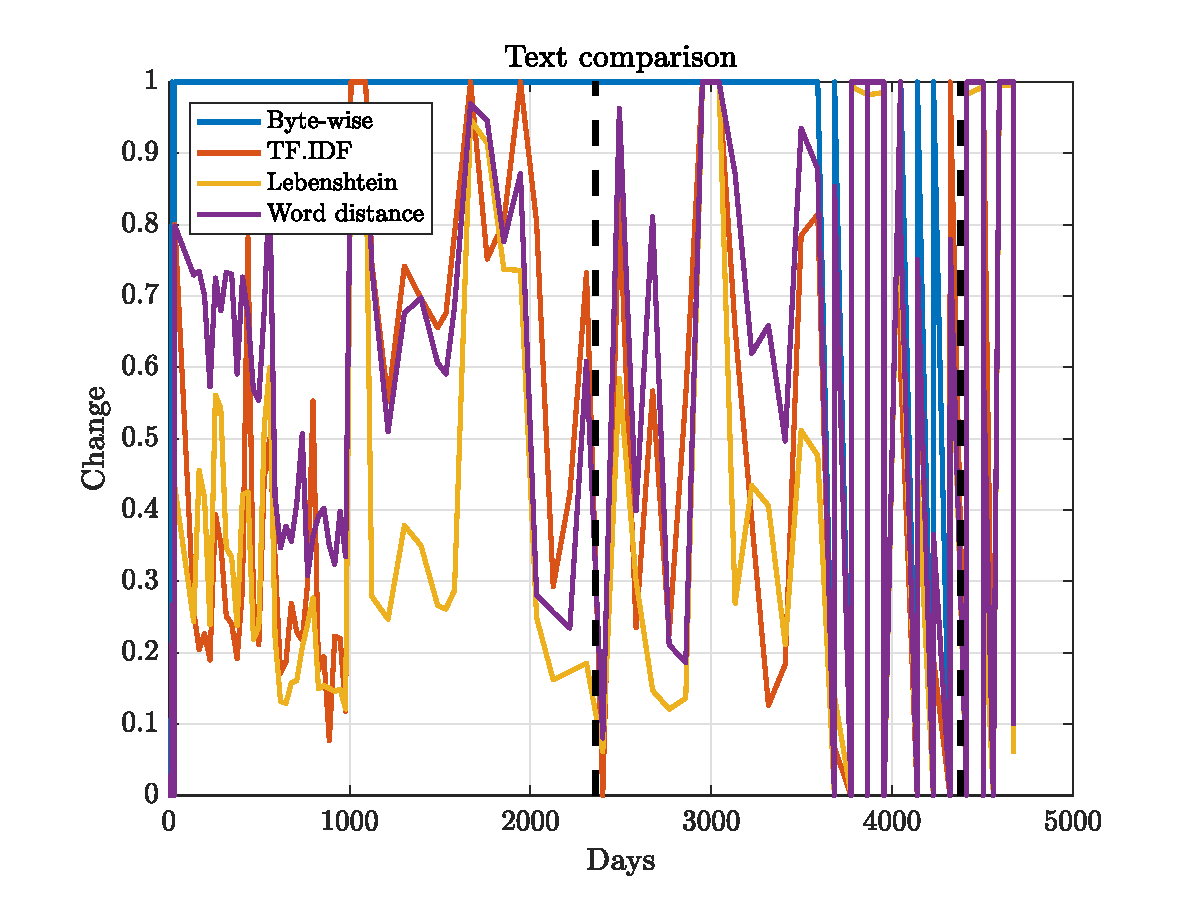
\includegraphics[width=70mm]{report-images/text_results}}
\subfigure[Results of the image comparison (the missing data corresponds to wayback rendering fails).]{\label{fig:image}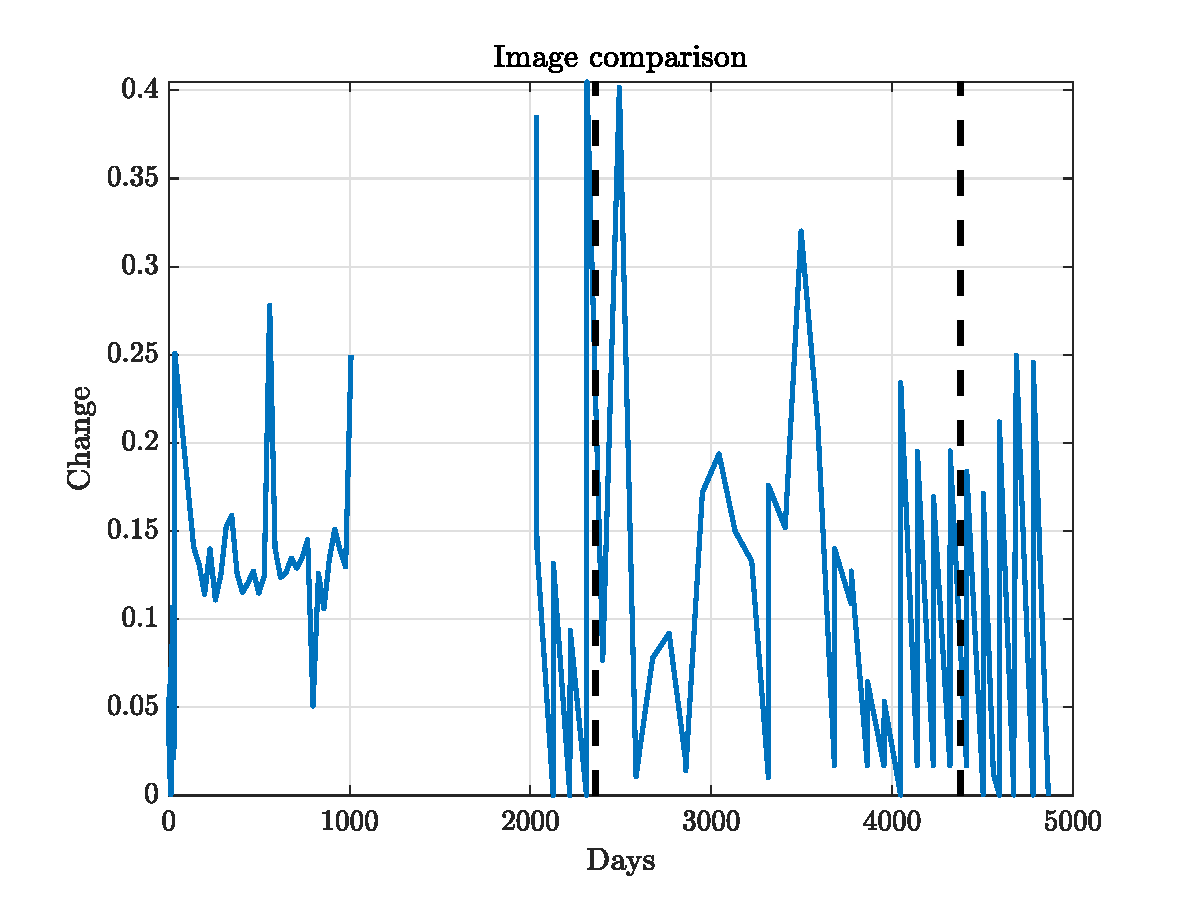
\includegraphics[width=70mm]{report-images/image_results}}
\subfigure[Results of the link comparison (plotted for the period where we had data available).]{\label{fig:links}\includegraphics[width=70mm]{report-images/link_results}}
\subfigure[Results from text comparison, link comparison, and image comparison on the same axis. Text metric used in this plot is word distance.]{\label{fig:all}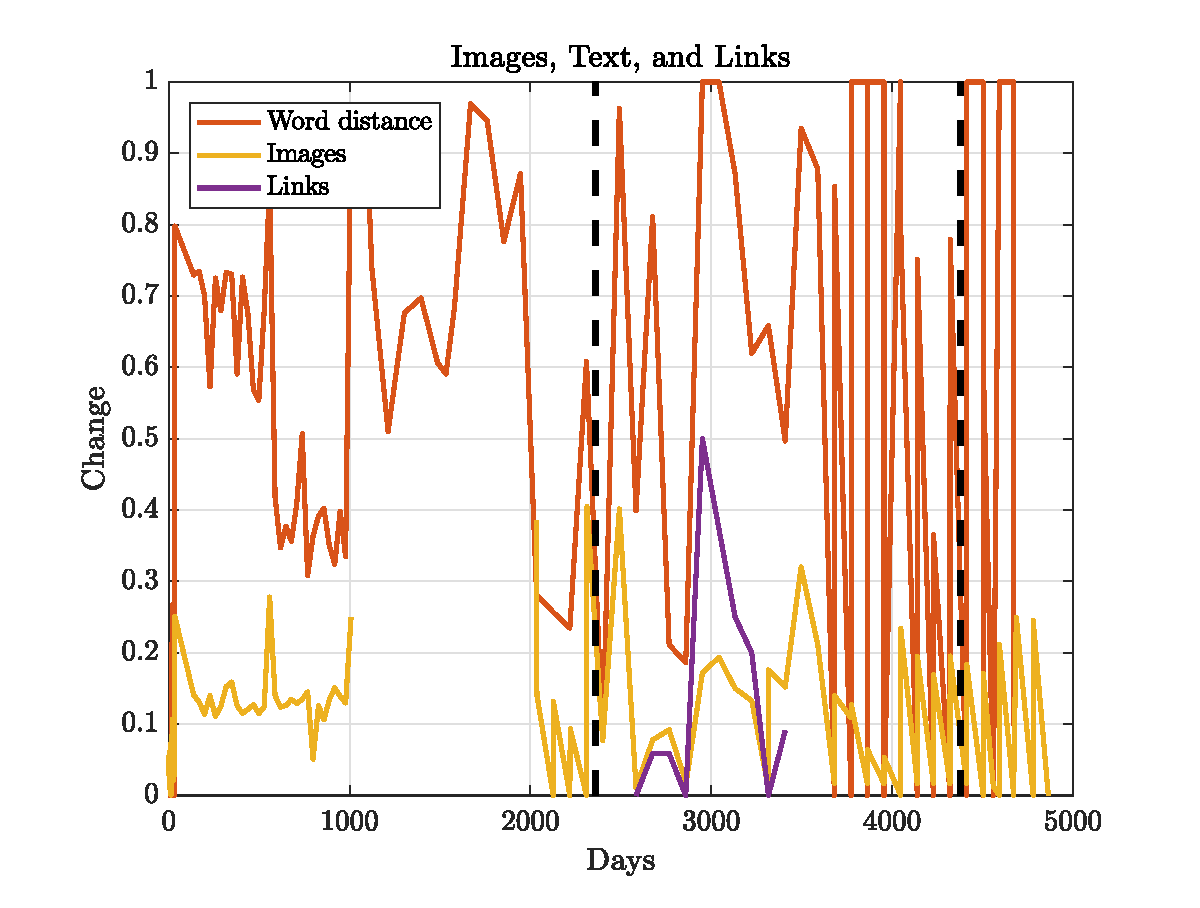
\includegraphics[width=70mm]{report-images/all_results_comparison}}
\caption{Preliminary results using data generated from \texttt{www.ndp.ca}. The dashed black lines correspond to the two days during this period when the NDP leadership changed.}
\label{fig:results}
\end{figure}

\section{Conclusion}
\vspace{-2mm}
 This report outlines some preliminary findings at the Industrial Problem Solving Workshop 2019 at the Fields Institute, Toronto.
 We explore the quantification of website domain change over time through the analysis of text, link, and thumbnail change.
 We believe that these different metrics have different uses depending on the domain being analysed and the type of change that is trying to be detected.
 For example, news websites update their text content every day, so any metric reliant solely on text may be over-sensitive.
 On the other hand, governmental websites may only update their text at times of relevant policy or leadership change.
 The results in Figure \ref{fig:all} demonstrate, for the data analysed in this report (\texttt{www.ndp.ca}), that the metrics agree qualitatively on the locations of large and small change.
 This implies some consistency between the metrics and suggests that with further work and added sophistication to the metrics, these techniques could be used to successfully indicate significant changes in web domains.
 An extension to this work could include combining the three different metrics in a weighted sum, where the weightings for each metric could be chosen based on the content being analysed, and by using these results to predict when a domain is next going to have a large change.

\bibliography{bibliography}
\bibliographystyle{ieeetr}


\end{document}
